\documentclass[11pt, a4paper, twoside, headsepline]{scrreprt}
\usepackage{scrpage2} 
%\usepackage{perpage} %make footnotes per page
%\MakePerPage{footnote}
\usepackage[utf8]{inputenc}
\usepackage[swedish,english]{babel}
\usepackage[T1]{fontenc}
\usepackage{lmodern}
\usepackage{amsmath}
\usepackage{fixmath}
\usepackage{graphicx}
%\usepackage{xcolor}
%\usepackage{textcomp}
\usepackage[usenames,dvipsnames]{color}
\usepackage[small,font=it]{caption}
\usepackage{amssymb}
\usepackage{units}
\usepackage{upgreek}
\usepackage{icomma}
%\usepackage{pdfpages}
\usepackage{cite}
\usepackage{listings}
\usepackage{units}
%\usepackage[sc]{titlesec}
%\usepackage{fancyhdr}
\usepackage[breakall,fit]{truncate}
\usepackage[intoc,refpage]{nomencl}
\usepackage{lettrine}
\usepackage{geometry}
\usepackage{eso-pic}
\usepackage{titling}
\usepackage{multirow}
\usepackage{chngcntr}
\usepackage{amsthm}
\usepackage{subfig}
\usepackage{lmodern}
\usepackage{afterpage}
\usepackage{floatpag,mwe}

\newcommand{\floor}{\mathrm{floor}}

\setkomafont{disposition}{\bfseries}

\renewcommand{\headfont}{\fontsize{12}{12}\selectfont\normalfont\slshape}

    \makeatletter
    \renewcommand{\@makechapterhead}[1]{%
    \vspace*{50 pt}%
    {\setlength{\parindent}{0pt} \raggedright \normalfont
    \bfseries\Huge\thechapter.\ \, #1
    \par\nobreak\vspace{40 pt}}}
    \makeatother






\usepackage{upref}
\newcommand{\footnoteindex}[1]{\setcounter{footnote}{#1}\addtocounter{footnote}{-1}\footnotemark}
\newcommand{\footnoteref}[1]{Footnote #1}



\newcommand{\backgroundpic}[3]{%
\put(#1,#2){
		\parbox[b][\paperheight]{\paperwidth}{%
			\centering
			\includegraphics[width=\paperwidth,height=\paperheight,keepaspectratio]{#3}
			\vfill
}}}

\newcommand{\mail}[1]{\href{mailto:#1}{\nolinkurl{#1}}}

%\pagestyle{fancy}
%\lhead{\truncate{16em}{\fontsize{10}{11}\selectfont\rightmark}}
%\rhead{\truncate{20em}{\fontsize{10}{11}\selectfont\leftmark}}
%\lhead{\rightmark}
%\rhead{\leftmark}
%\setlength{\headheight}{15pt}

%%% Closed square root
\usepackage{letltxmacro}
\makeatletter
\let\oldr@@t\r@@t
\def\r@@t#1#2{%
\setbox0=\hbox{$\oldr@@t#1{#2\,}$}\dimen0=\ht0
\advance\dimen0-0.2\ht0
\setbox2=\hbox{\vrule height\ht0 depth -\dimen0}%
{\box0\lower0.4pt\box2}}
\LetLtxMacro{\oldsqrt}{\sqrt}
\renewcommand*{\sqrt}[2][\ ]{\oldsqrt[#1]{#2}}
\makeatother
%%%

%%%
\newcounter{myfootnote}
\makeatletter
\@addtoreset{equation}{myfootnote}
\makeatother
\newcounter{myequation}
\makeatletter
\@addtoreset{equation}{myequation}
\makeatother
% Resetting the equation counter is done by stepping myequation, so use \stepcounter{myequation} instead of \setcounter{equation}{0}
% Else, hyperref fails
\newcounter{myfigure}
\makeatletter
\@addtoreset{figure}{myfigure}
\makeatother
\newcounter{mytable}
\makeatletter
\@addtoreset{table}{mytable}
\makeatother
%%%


%\renewcommand\headheight{14pt}


\usepackage[bookmarks, unicode=true, pdftitle={EventGenerators}, pdfauthor={Stefan Buller}, colorlinks=true, linkcolor=black, citecolor=black, urlcolor=black]{hyperref} %assumes black text!

\usepackage[all]{hypcap}
\usepackage[intoc,refpage]{nomencl}
\renewcommand{\nomname}{Glossary} % rename nomenclature
\renewcommand{\nomlabel}[1]{\textbf{#1}}
\makenomenclature

\def\figureautorefname{Figure}
\def\chapterautorefname{Section}
\def\sectionautorefname{Section}
\def\subsectionautorefname{Section}
\def\subsubsectionautorefname{Section}
\newcommand{\subfigureautorefname}{\figureautorefname}

\newenvironment{myenumerate}{%
  \edef\backupindent{\the\parindent}%
  \enumerate%
  \setlength{\parindent}{\backupindent}%
}{\endenumerate}


\makeatletter
\newenvironment{tablehere}
  {\def\@captype{table}}
  {}

\newenvironment{figurehere}
  {\def\@captype{figure}}
  {}
\makeatother

\newcommand{\ordo}[1]{{\cal O}\left( #1 \right)}
\newcommand{\im}{\ensuremath{\mathrm{i}}}
\newcommand{\e}{\ensuremath{\mathrm{e}}}
\renewcommand{\d}{\ensuremath{\mathrm{d}}}

\newcommand{\bra}[1]{\langle #1 \mid}
\newcommand{\ket}[1]{\mid #1 \rangle}
\renewcommand{\vec}[1]{\boldsymbol{#1}}

\newcommand{\chem}[2]{\mathrm{#1}_{#2}}
\newcommand{\dfn}[2]{\emph{#1}\footnote{#2}}
\newcommand{\abbrev}[2]{\emph{#1} (#2)}
\newcommand{\E}[1]{\ensuremath{\mathrm{E}[#1]}}

\newcommand{\rtb}{\ensuremath{\text{R}^3\text{B}}}
\newcommand{\me}{\ensuremath{\mathcal{M}}}

%\newcommand{\prgname}[1]{\textsc{#1}}
%to make smallcaps work in \section, etc. normally a problem because no bold sc
%texorpdfstring to make hyperref give proper side-bar clicky!
 \usepackage{relsize}
  \newcommand{\prgname}[1]{\texorpdfstring{\textsmaller{\MakeUppercase{#1}}}{\textsc{#1}}}


\newcommand{\pM}{\mathrel{\raise -2.2pt \hbox{\tiny(\,}\!
                 \raise 2pt \hbox{+}
                 \settowidth {\dimen03} {+}
                 \hskip-\dimen03
                 \raise -3.4pt \hbox {$-$}
                 \!\raise -2.2pt \hbox{\tiny{\,)}}}}

\newcommand{\codename}{\prgname{Codez}}
\newcommand{\nucl}[3]{
\ensuremath{
\phantom{\ensuremath{^{#1}_{#2}}}
\llap{\ensuremath{^{#1}}}
\llap{\ensuremath{_{\rule{0pt}{.75em}#2}}}
\mbox{#3}
}
}

\title{Event Generator for \rtb{}}
\author{Stefan Buller}
\date{\today}


\begin{document}
% Chalmers title page
\begin{titlepage}
\AddToShipoutPicture{\backgroundpic{-4}{56.7}{titlepageabstract/frontpage}}
\mbox{}
%\vspace{10cm}
\scalebox{0.12}{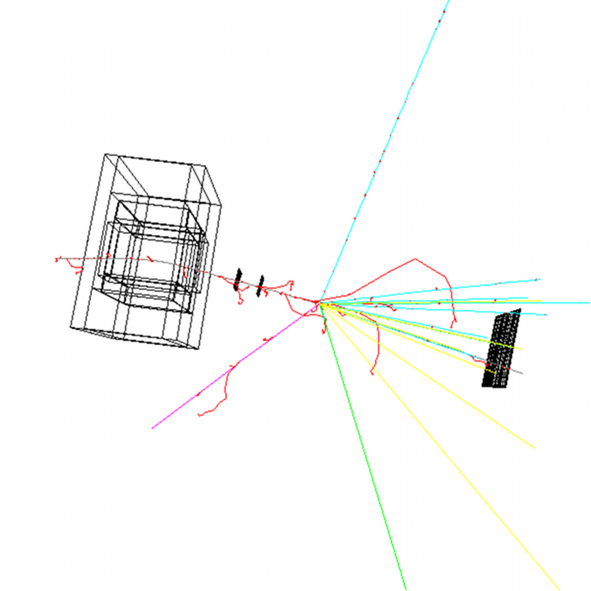
\includegraphics{titlepageabstract/titlefig2.pdf}}
\vfill
%\vspace*{-12cm}
\addtolength{\voffset}{2cm}
\begin{flushleft}
%\vspace*{3cm}
	{\noindent \LARGE{Event Generator for \rtb{}} \\[0.3cm]
	\emph{\Large Master's Thesis in Physics and Astronomy} \\[.8cm]
	
	\Large{STEFAN BULLER}\\[.8cm]
	
	{\Large Department of Fundamental Physics \\
	\textsc{Chalmers University of Technology} \\
	Gothenburg, Sweden 2015 \\
%	Master's Thesis 2011:1\\
	} 
	}
\end{flushleft}
\end{titlepage}
\ClearShipoutPicture
% End Chalmers title page
\pagestyle{empty}
\clearpage
\mbox{}
\clearpage
\thispagestyle{empty}

\thispagestyle{empty}
\begin{titlepage}

\begin{center}
\vspace*{0.5cm}
\huge{\textbf{\thetitle }}
\vspace*{1.5cm}

\Large{\textsc{Master's Thesis}}\\
\vspace*{1cm}
\large{\textsc {by}}\\
\vspace*{0.4cm}
\LARGE{\theauthor}\\
\vspace*{1.2cm}
\Large{\textsc{Supervisors:}}\\
\vspace*{0.4cm}
\LARGE{Andreas Heinz}\\
\vspace*{1.0cm}
\Large{\textsc{Examiners:}}\\
\vspace*{0.4cm}
\LARGE{Thomas Nilsson}
\vfill
\large{Department of Fundamental Physics \\
	Chalmers University of Technology \\
	Gothenburg, Sweden 2015}
\end{center}

\end{titlepage}
\clearpage
\noindent EventGenerators\\
\noindent Stefan Buller (\href{mailto:bstefan@student.chalmers.se}{bstefan@student.chalmers.se})\\\\
\copyright Stefan Buller, 2015.\\\\
FUFX03  - Master's thesis at Fundamental Physics\\
Supervisor: Andreas Heinz\\
Examiner: Thomas Nilsson\\\\
Department of Fundamental Physics\\
Chalmers University of Technology\\
SE-412 96 Göteborg\\
Sweden\\
+46 (31) 772 1000\\\\
Printed by Chalmers Reproservice\\
Göteborg, Sweden 2015
 
\vfill
\noindent{\bf Cover:} The prefered decay modes for various nuclei at an excitation energy of \unit[15]{MeV}, according to the code developed in this project. A red box signifies that the nucleus preferentially decays by emitting a proton, while a blue box means that neutron emission is the most common decay mode. Cyan boxes corresponds to nuclei who deexcite primarily by emitting an alpha particle.
\clearpage
%\begin{minipage}[t][0.50\textheight]{\textwidth}
\subsection*{\centering Abstract}
{\fontsize{10}{11}\selectfont 
This thesis describes various models implemented in a code to simulate nuclear reactions that go through a compound nucleus state, an intermediate excited state long lived enough that the nucleus has time to reach equilibrium between each subsequent decay. This implies that the decay is effectively characterized by macroscopically conserved quantities such as the excitation energy $E^*$ and its spin $J$, in addition to the proton and neutron number, $Z$ and $N$, respectively.

Specifically, the reactions under consideration are quasi-elastic scattering reactions, in which the collision is modeled as taking place between essentially free nucleons or clusters in the target and projectile. A Feynman diagram formalism is used to describe this first, fast knock-out reaction.
The unaffected nucleons in the projectile will then form an excited compound nucleus, and the final reaction products are determined by decaying this compound system. 

The codes to simulate the initial fast reaction and subsequent decay are separate programs. Results are presented regarding the prefered decay modes of nuclei with a given excitation energy, utilizing the decay part of the code. The results obtained for an excitation energy of $\unit[20]{MeV}$ were compared with the output of another program, \prgname{Talys}, for nuclei with $Z\in [10,90]$ and $N \in [10,130]$. 

Finally, the quasi-elastic scattering code and the compound nucleus deexcitation code were coupled in order to allow the code to be used as an event generator. The output of the event generator was used in simulations to benchmark the performance of the addback algorithm used to determine gamma energies and multiplicites from actual experimental data. The tentative results indicate that the addback algorithm is unable to identify the number of $\gamma$-rays emitted in the reaction, although further investigations are needed to arrive at a conclusive result.
}
%\end{abstract}
%\end{minipage}
%\vspace{-3cm}

\selectlanguage{english}
\thispagestyle{empty}

\chapter*{Acknowledgements}
%Lorem ipsum dolor sit amet, consectetur adipisicing elit, sed do eiusmod tempor incididunt ut labore et dolore magna aliqua. Ut enim ad minim veniam, quis nostrud exercitation ullamco laboris nisi ut aliquip ex ea commodo consequat. Duis aute irure dolor in reprehenderit in voluptate velit esse cillum dolore eu fugiat nulla pariatur. Excepteur sint occaecat cupidatat non proident, sunt in culpa qui officia deserunt mollit anim id est laborum. 

\thispagestyle{empty}
This project would not have started or finished without Andreas Heinz, who both suggested the topic and provided support and supervision throughout this project.

The \prgname{Talys} simulations, which were used to partially compare the output of the code, would obviously not have been possible without the \prgname{Talys} team. In particular, I am indepted to Arjan Koning for being helpful over mail, providing me with the latest version of \prgname{Talys}, and for adding a \prgname{Talys} keyword that enabled me to do the comparison between the emission spectra of my program and \prgname{Talys}.

Also good at alleviating technology related pain is Håkan Johansson, who (mostly) has kept the computers at the subatomic physics group happy.

On the few occasions when the computers weren't happy, I could usually blame Simon Lindberg, who -- in addition to tormenting the intranet -- inspired me to have a look at gamma-multiplicites and explained the addback routine used to analyze the energy deposits in the Crystal Ball detector.

Last but not least, I would like to thank the entire subatomic physics group for bearing with me and making me feel welcome -- and the University for all the cake.
\\[1cm]

\hfill Stefan Buller, Gothenburg, June 2015
\clearpage
\pagenumbering{roman}



\selectlanguage{english}

